% DO NOT COMPILE THIS FILE DIRECTLY!
% This is included by the other .tex files.

\lstdefinestyle{bash}{ %
  backgroundcolor=\color{black!85},   % choose the background color; you must add \usepackage{color} or \usepackage{xcolor}; should come as last argument
  basicstyle=\footnotesize\color{mywhite},        % the size of the fonts that are used for the code
  breakatwhitespace=false,         % sets if automatic breaks should only happen at whitespace
  breaklines=true,                 % sets automatic line breaking
  captionpos=b,                    % sets the caption-position to bottom
  commentstyle=\color{mygreen},    % comment style
  deletekeywords={...},            % if you want to delete keywords from the given language
  escapeinside={\%*}{*)},          % if you want to add LaTeX within your code
  extendedchars=true,              % lets you use non-ASCII characters; for 8-bits encodings only, does not work with UTF-8
  frame=single	                   % adds a frame around the code
  keepspaces=true,                 % keeps spaces in text, useful for keeping indentation of code (possibly needs columns=flexible)
  keywordstyle=\color{white}\bfseries,       % keyword style
  language=bash,                 % the language of the code
  morekeywords={*,$,git, clone,... },           % if you want to add more keywords to the set
  numbers=left,                    % where to put the line-numbers; possible values are (none, left, right)
  numbersep=5pt,                   % how far the line-numbers are from the code
  numberstyle=\tiny\color{mywhite}, % the style that is used for the line-numbers
  rulecolor=\color{black},         % if not set, the frame-color may be changed on line-breaks within not-black text (e.g. comments (green here))
  showspaces=false,                % show spaces everywhere adding particular underscores; it overrides 'showstringspaces'
  showstringspaces=false,          % underline spaces within strings only
  showtabs=false,                  % show tabs within strings adding particular underscores
  stepnumber=1,                    % the step between two line-numbers. If it's 1, each line will be numbered
  stringstyle=\color{mymauve},     % string literal style
  tabsize=2,	                   % sets default tabsize to 2 spaces
  title=\lstname                   % show the filename of files included with \lstinputlisting; also try caption instead of title
}

\begin{frame}[t,plain]
\titlepage
\end{frame}

\section{Introduction}
\begin{frame}
        \frametitle{Concepts - Deep Web}
        \begin{itemize}
                \item {\bf Deep Web} is the part of World Wide Web not indexed or directly accessible by standard web search-engines;
                \item This can be content hidden from {\bf crawlers} by requiring a specific access and this can includes private social media, password-protected forums or content protected
                        by different measures such as paywalls or specific security interface to access the information;
                \item A large portion of content accessible via Internet is part of the deep web\footnote{also called invisible web, hidden web or non-indexed web}.
        \end{itemize}
        \note[item]{There is a huge misconception about the difference between the darknet and deep web. The differences are important because it's two different aspects which can be related to each other.}
\end{frame}

\begin{frame}
        \frametitle{Concepts - darknet}
        \begin{itemize}
                \item {\bf Darknet} is an overlay network running on top of Internet requiring specific software to access the network and its services;
                \item Tor, I2P and Freenet are the most commonly used ones. Many are used for hidden services access and some for proxy access to the Internet;
		\item There are {\bf legitimate use-cases} for such network but also many {\bf illegal or criminal usage}.
        \end{itemize}
\end{frame}

\begin{frame}
	\frametitle{Lifecycle of collection and analysis}
	\center
\tikzstyle{startstop} = [rectangle, rounded corners, minimum width=3cm, minimum height=0.8cm,text centered, draw=black, fill=white!10]
\tikzstyle{io} = [trapezium, trapezium left angle=70, trapezium right angle=110, minimum width=3cm, minimum height=1cm, text centered, draw=black, fill=blue!30]
\tikzstyle{arrow} = [thick,->,>=stealth]
	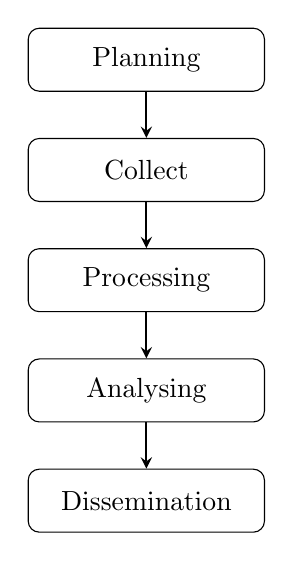
\begin{tikzpicture}[node distance=1.4cm]

\node (start) [startstop] {Planning};
\node (collect) [startstop, below of =start] {Collect};
\node (processing) [startstop, below of =collect] {Processing};
\node (analysing) [startstop, below of=processing] {Analysing};
\node (dissemination) [startstop, below of=analysing] {Dissemination};
\draw [arrow] (start) -- (collect);
\draw [arrow] (collect) -- (processing);
\draw [arrow] (processing) -- (analysing);
\draw [arrow] (analysing) -- (dissemination);
%\draw [arrow] (analysing) |- (collect);
\end{tikzpicture}

\end{frame}

\begin{frame}
        \frametitle{Collecting, processing and analysing content - web pages}
        \begin{itemize}
		\item Building a search engine on the web is a challenging task because:
        	\begin{itemize}
			\item it has to crawl webpages,
			\item it has to to make sense of {\bf unstructured data},
			\item it has to {\bf index} these data,
			\item it has to provide a way to retrieve data and structure data (e.g. correlation).
        	\end{itemize}
		\item Doing so on Tor is even more challenging because:

        	\begin{itemize}
			\item services don't always want to be found,
			\item parts of the dataset have to be discarded.
        	\end{itemize}
	\item in each case, it requires a lot of bandwidth, storage and computing power.
        \end{itemize}
\end{frame}

\begin{frame}
        \frametitle{Collecting, processing and analysing content - structured data}
        \begin{itemize}
		\item Some data are structured and are easy to process:
        	\begin{itemize}
			\item metadata!
			\item API responses.
        	\end{itemize}
		\item Some even provide cryptographic evidences:
			        \begin{itemize}

         \item authentication mechanisms between peers,
         \item OpenGPG can leak a lot of metadata
        \begin{itemize}
          \item key ids,
          \item subject of email in thunderbird,
        \end{itemize}
          \item Bitcoin's Blockchain is public,
          \item pivoting on these data with external sources yields interesting results.
        \end{itemize}
        \end{itemize}
\end{frame}

\section{AIL design Objectives}
\begin{frame}
\frametitle{Objectives of the session}
    \begin{itemize}
        \item Show how to use and extend an open source tool to monitor web pages, pastes, forums and hidden services
        \item Explain challenges and the design of the AIL open source framework
        \item Review different {\bf collection mechanisms} and {\bf sources}
        \item Learn how to create new modules
        \item Learn how to use, install and start AIL
        \item {\bf Supporting investigation using the AIL framework} and including it in cyber threat intelligence lifecycle
    \end{itemize}
\end{frame}

\section{AIL Framework}
\begin{frame}
    \frametitle{From a requirement to a solution: AIL Framework}
    \large{History:}
    \begin{itemize}
        \item AIL initially started as an \textbf{internship project} (2014) to evaluate the feasibility to automate the analysis of (un)structured information to find leaks.
        \item In 2019, AIL framework is an \textbf{open source software} in Python. The software is actively used (and maintained) by CIRCL and many organisations.
        \item In 2020, AIL framework is now a complete project called \textbf{ail project}\footnote{\url{https://github.com/ail-project/}}.
    \end{itemize}
\end{frame}

\section{Capabilities Overview}

\begin{frame}
    \frametitle{Common usage}
        \begin{itemize}
                \item {\bf Check} if mail/password/other sensitive information (terms tracked) leaked
                \item {\bf Detect} reconnaissance of your infrastructure
                \item {\bf Search} for leaks inside an archive
                \item {\bf Monitor} and crawl websites
        \end{itemize}
\end{frame}

\begin{frame}
    \frametitle{Support CERT/CSIRTs and Law Enforcement activities}
        \begin{itemize}
            \item Proactive investigation: leaks detection
            \begin{itemize}
		        \item List of emails and passwords
		        \item Leaked database
		        \item AWS Keys
		        \item Credit-cards
		        \item PGP private keys
		        \item Certificate private keys
		    \end{itemize}
		    \item Feed Passive DNS or any passive collection system
		    \item CVE and PoC of vulnerabilities most used by attackers
		\end{itemize}
\end{frame}

\begin{frame}
    \frametitle{Support CERT/CSIRTs and Law Enforcement activities}
    	\begin{itemize}
		    \item Website monitoring
		    	\begin{itemize}
				    \item monitor booters
                    \item Detect encoded exploits (WebShell, malware encoded in Base64...)
				    \item SQL injections
		    	\end{itemize}
		    \item Automatic and manual submission to threat sharing and incident
response platforms
			\begin{itemize}
				\item MISP
				\item TheHive
			\end{itemize}
		    \item Term/Regex/Yara monitoring for local companies/government
        \end{itemize}
\end{frame}

\begin{frame}
    \frametitle{Sources of leaks: Paste monitoring}
    \begin{itemize}
        \item Example: \url{https://gist.github.com/}
            \begin{itemize}
                \item Easily storing and sharing text online
                \item Used by programmers and legitimate users
                \item[] $\to$ Source code \& information about configurations
            \end{itemize}
        \pause
        \item Abused by attackers to store:
            \begin{itemize}
                \item List of vulnerable/compromised sites
                \item Software vulnerabilities (e.g. exploits)
                \item Database dumps
                \item[] $\to$ User data
                \item[] $\to$ Credentials
                \item[] $\to$ Credit card details
                \item More and more ...
            \end{itemize}
    \end{itemize}
\end{frame}

\begin{frame}
        \frametitle{Why so many leaks?}
        \begin{itemize}
                \item Economical interests (e.g. Adversaries promoting services)
                \item Ransom model (e.g. To publicly pressure the victims)
                \item Political motives (e.g. Adversaries showing off)
                \item Collaboration (e.g. Criminals need to collaborate)
                \item Operational infrastructure (e.g. malware exfiltrating information on a pastie website)
                \item Mistakes and errors
        \end{itemize}
\end{frame}


\begin{frame}
    \frametitle{Are leaks frequent?}
    \begin{center}
    \Large{Yes!}\\ and we have to deal with this as a CSIRT.
    \end{center}

    \begin{itemize}
            \item {\bf Contacting companies or organisations} who did specific accidental leaks
            \item {\bf Discussing with media} about specific case of leaks and how to make it more practical/factual for everyone
            \item Evaluating the economical market for cyber criminals (e.g. DDoS booters\footnote{\url{https://github.com/D4-project/}} or reselling personal information - reality versus media coverage)
            \item Analysing collateral effects of malware, software vulnerabilities or exfiltration
    \end{itemize}

    \begin{center}
    $\rightarrow$ And it's important to detect them automatically.
    \end{center}
\end{frame}

\begin{frame}
    \frametitle{Paste monitoring at CIRCL: Statistics}
    \begin{itemize}
        \item Monitored paste sites: 27
            \begin{itemize}
                \item \textit{gist.github.com}
                \item \textit{ideone.com}
                \item \textit{...}
            \end{itemize}
    \end{itemize}
    \begin{table}[h]
		\centering
		\begin{tabular}{|lrrr|}
		    \hline
		    \rowcolor{lightgray} & 2016 & 2017 & 08.2018\\
		    Collected pastes & 18,565,124 & 19,145,300 & 11,591,987 \\
		    Incidents & 244 & 266 & 208\\
		    \hline
		\end{tabular}
		\caption{Pastes collected and incident\footnote{\url{http://www.circl.lu/pub/tr-46}} raised by CIRCL}
		\label{circlStats}
	\end{table}
\end{frame}


\section{Current capabilities}

\begin{frame}
    \frametitle{AIL Framework: Current capabilities}
    \begin{itemize}
        \item Extending AIL to add a new {\bf analysis module} can be done in 50 lines of Python
        \item The framework {\bf supports multi-processors/cores by default}. Any analysis module can be started multiple times to support faster processing during peak times or bulk import
        \item \textbf{Multiple} concurrent \textbf{data input}
        \item Tor Crawler (handle cookies authentication)
    \end{itemize}
\end{frame}

\begin{frame}
    \frametitle{AIL Framework: Current features}
    \begin{itemize}
        \item Extracting \textbf{credit cards numbers, credentials, phone numbers, ...}
        \item Extracting and validating potential \textbf{hostnames}
        \item Keeps track of \textbf{duplicates}
        \item Submission to threat sharing and incident response platform (\textbf{MISP} and \textbf{TheHive})
        \item \textbf{Full-text indexer} to index unstructured information
        \item \textbf{Tagging} for classification and searches
        \item Terms, sets, regex and YARA \textbf{tracking and occurences}
        \item Archives, files and raw \textbf{submission} from the UI
        \item PGP, Cryptocurrency, Decoded (Base64, ...) and username Correlation
        \item And many more
    \end{itemize}
\end{frame}

\begin{frame}
    \frametitle{Terms Tracker}
        \begin{itemize}
            \item Search and monitor specific keywords/patterns
            \begin{itemize}
                \item Automatic Tagging
                \item Email Notifications
            \end{itemize}
            \item Track Term
            \begin{itemize}
                \item ddos
            \end{itemize}
            \item Track Set
            \begin{itemize}
                \item booter,ddos,stresser;2
            \end{itemize}
            \item Track Regex
            \begin{itemize}
                \item circl\textbackslash.lu
            \end{itemize}
            \item YARA rules
                \begin{itemize}
                \item https://github.com/ail-project/ail-yara-rules
            \end{itemize}
        \end{itemize}
\end{frame}

\begin{frame}
    \frametitle{Terms Tracker}
        \begin{figure}
            \includegraphics[scale=0.22]{images/term-tracker.png}
        \end{figure}
\end{frame}

\begin{frame}
    \frametitle{YARA Tracker}
        \begin{figure}
            \includegraphics[scale=0.22]{screenshot/term-tracker-yara.png}
        \end{figure}                                                                                   
\end{frame}

\begin{frame}
    \frametitle{Terms Tracker - Practical part}
        \begin{itemize}
            \item \textbf{Create and test} your own tracker
            \includegraphics[scale=0.3]{images/term-tracker-create.png}
        \end{itemize}
\end{frame}

\begin{frame}
    \frametitle{Recon and intelligence gathering tools}
        \begin{itemize}
            \item {\bf Attacker also share informations}
            \item Recon tools detected: 94
            \begin{itemize}
                \item sqlmap
                \item dnscan
                \item whois
                \item msfconsole (metasploit)
                \item dnmap
                \item nmap
                \item ...
            \end{itemize}
        \end{itemize}
\end{frame}


\begin{frame}
    \frametitle{Recon and intelligence gathering tools}
        \begin{figure}
            \includegraphics[scale=0.4]{images/recon-paste.png}
        \end{figure}
\end{frame}


\begin{frame}
    \frametitle{Decoder}
    \begin{itemize}
        \item Search for encoded strings
            \begin{itemize}
                \item Base64
                \item Hexadecimal
                \item Binary
            \end{itemize}
        \item Guess Mime-type
        \item Correlate paste with decoded items
    \end{itemize}
\end{frame}                                                                                         


\begin{frame}
    \frametitle{Decoder:}
    \centerline{
        \includegraphics[scale=0.23]{images/decoded-dos.png}
    }
\end{frame}

\begin{frame}
        \frametitle {Crawler}
        \begin{itemize}
                \item Crawlers are used to navigate on regular website as well as .onion addresses (via automatic extraction of urls or manual submission)
                \item Splash ("scriptable" browser) is rending the pages (including javascript) and produce screenshots (HAR archive too)
        \end{itemize}
\begin{figure}[h]
    \centering
    \begin{tikzpicture}[scale=1.0,
        mymatrix/.style={matrix of nodes, nodes=typetag, row sep=1em},
        mycontainer/.style={draw=gray, inner sep=1ex},
        typetag/.style={draw=gray, inner sep=1ex, anchor=west},
        title/.style={draw=none, color=gray, inner sep=0pt}
    ]

    %styles 
    \tikzstyle{Docker}=[ellipse,draw,align=center]
    \tikzstyle{AIL}=[rectangle,draw, align=center, fill={rgb:red,1;green,2;blue,5}]
    \tikzstyle{Splash}=[rectangle,draw, align=center, fill={rgb:red,1;green,2;blue,5}]
    \tikzstyle{commu}=[<->,>=latex,very thick]

    %nodes 
    \matrix[mymatrix] (mx1) at (0, 0) {
        |[title]|Docker container \\
        Splash \\
    };
    \matrix[mymatrix, right=of mx1.north east, matrix anchor=north west] (mx2) {
    %\matrix[mymatrix] (mx2) at (1, 0) { 
        |[title]|... \\ 
    }; 
    \matrix[mymatrix, right=of mx2.north east, matrix anchor=north west] (mx3) { 
    %\matrix[mymatrix] (mx3) (2, 0){ 
        |[title]|Docker container \\ 
        Splash \\ 
    }; 
 
    \node[mycontainer, fit=(mx1)] (c1) {}; 
    \node[mycontainer, fit=(mx2)] (c2) {}; 
    \node[mycontainer, fit=(mx3)] (c3) {}; 
 
    %\node[AIL, below=of mx2.south, matrix anchor=north] (ail) {\color{white}AIL-framework}; 
    \node[AIL, below= 3cm of mx2.south, matrix anchor=north] (ail) {\color{white}AIL-framework}; 
 
    %arraws 
    \draw[commu] (ail)--(c1); 
    \draw[commu] (ail)--(c2); 
    \draw[commu] (ail)--(c3); 
 
 
    \end{tikzpicture}                                                                                                                                                                                                       
\end{figure}
\end{frame}

\begin{frame}
    \frametitle{Crawler}
    \begin{itemize}
    \item[] How a domain is crawled by default
        \begin{enumerate}
            \item Fetch the first url
            \item Render javascript (webkit browser)
            \item Extract all urls
            \item Filter url: keep all url of this domain
            \item crawl next url (max depth = 1)
        \end{enumerate}
    \end{itemize}
\end{frame}

\begin{frame}
    \frametitle{Crawler: Cookiejar}
    Use your cookies to login and bypass captcha
    \centerline{
        \includegraphics[scale=0.23]{screenshot/crawler-cookiejar-edit.png}
    }
\end{frame}

\begin{frame}
    \frametitle{Crawler: Cookiejar}
    \centerline{
        \includegraphics[scale=0.23]{screenshot/crawler-cookiejar-domain-crawled.png}
    }
\end{frame}

\begin{frame}
    \frametitle{Correlations and relationship}
    \begin{figure}
        \includegraphics[scale=0.18, angle=0]{images/ail-correlation.png}
    \end{figure}
\end{frame}

\section{Live demo!}

\begin{frame}
    \frametitle{Example: Dashboard}
    \begin{figure}
        \includegraphics[scale=0.18, angle=0]{screenshot/dashboard.png}
    \end{figure}
\end{frame}


\begin{frame}
    \frametitle{Example: Text search}
    \begin{figure}
        \includegraphics[scale=0.3, angle=0]{images/ail_02.png}
    \end{figure}
\end{frame}

\begin{frame}
    \frametitle{Example: Items Metadata (1)}
    \begin{figure}
        \includegraphics[scale=0.21, angle=0]{images/ail_15.png}
    \end{figure}
\end{frame}

\begin{frame}
    \frametitle{Example: Items Metadata (2)}
    \begin{figure}
        \includegraphics[scale=0.28, angle=0]{images/ail_16.png}
    \end{figure}
\end{frame}

\begin{frame}
    \frametitle{Example: Items Metadata (3)}
    \begin{figure}
        \includegraphics[scale=0.28, angle=0]{images/ail_17.png}
    \end{figure}
\end{frame}

\begin{frame}
    \frametitle{Example: Browsing content}
    \begin{figure}
        \includegraphics[scale=0.3, angle=0]{images/ail_04.png}
    \end{figure}
\end{frame}


\begin{frame}
    \frametitle{Example: Browsing content}
    \begin{figure}
        \includegraphics[scale=0.3, angle=0]{images/ail_06.png}
    \end{figure}
\end{frame}
                                                                                                            
\begin{frame}
    \frametitle{Example: Search by tags}
    \begin{figure}
        \includegraphics[scale=0.26, angle=0]{images/ail_14.png}
    \end{figure}
\end{frame}

\section{MISP}

\begin{frame}
    \frametitle{MISP Taxonomies}
        \begin{itemize}
            \item {\bf Tagging} is a simple way to attach a classification to an event or anattribute.
            \item {\bf Classification must be globally used to be efficient.}
            \item Provide a set of already defined classifications modeling estimative language
            \item Taxonomies are implemented in a simple JSON format \footnote{\url{https://github.com/MISP/misp-taxonomies}}.
            \item Can be easily cherry-picked or extended
        \end{itemize}
\end{frame}

\begin{frame}
    \frametitle{Taxonomies useful in AIL}
        \begin{itemize}
            \item {\bf infoleak}: Information classified as being potential leak.
            \item {\bf estimative-language}: Describe quality and credibility of underlying sources, data, and methodologies.
            \item {\bf admiralty-scale}: Rank the reliability of a source and the credibility of an information
            \item {\bf fpf\footnote{Future of Privacy Forum}}: Evaluate the degree of identifiability of personal data and the types of pseudonymous data, de-identified data and anonymous data.
        \end{itemize}
\end{frame}

\begin{frame}
    \frametitle{Taxonomies useful in AIL}
        \begin{itemize}
            \item {\bf tor}: Describe Tor network infrastructure.
            \item {\bf dark-web}: Criminal motivation on the dark web.
            \item {\bf copine-scale\footnote{Combating Paedophile Information Networks in Europe}}: Categorise the severity of images of child sex abuse.
        \end{itemize}
\end{frame}

\begin{frame}
    \frametitle{threat sharing and incident response platforms}
    \centerline{
        \includegraphics[scale=0.14]{images/ail-project.png}
        \hskip 2em 
        $\longrightarrow$
        \hskip 2em
        \includegraphics[scale=0.8]{images/MISP.png}
    }

    \vskip 2em
    \textbf{Goal:} submission to threat sharing and incident
response platforms.
\end{frame}

\begin{frame}
    \frametitle{threat sharing and incident response platforms}
    \centerline{
        \includegraphics[scale=0.12]{images/ail-project.png}
        \hskip 2em
        $\longrightarrow$
        \hskip 2em
        \includegraphics[scale=0.8]{images/MISP.png}
    }

    \vskip 2em
    \begin{enumerate}
            \item Use infoleak taxonomy\footnote{\url{https://www.misp-project.org/taxonomies.html}}
        \item Add your own tags                                                                                                                                                                            
    \item Export AIL objects to MISP core format
    \item Download it or Create a MISP Event\footnote{\url{https://www.misp-standard.org/rfc/misp-standard-core.txt}}
    \end{enumerate}
\end{frame}

\begin{frame}
    \frametitle{MISP Export}
    \centerline{\includegraphics[scale=0.35]{screenshot/bitcoin-misp.png}}
\end{frame}

\begin{frame}
    \frametitle{MISP Export}
    \centerline{\includegraphics[scale=0.35]{screenshot/domain-misp.png}}
\end{frame}

\begin{frame}
    \frametitle{MISP Export}
    \centerline{\includegraphics[scale=0.25]{screenshot/misp-export.png}}
\end{frame}

\begin{frame}
    \frametitle{Automatic submission on tags}
    \centerline{\includegraphics[scale=0.25]{screenshot/tag_auto_export.png}}
\end{frame}


\section{API}

\begin{frame}[fragile]
AIL exposes a ReST API which can be used to interact with the back-end\footnote{\url{https://github.com/ail-project/ail-framework/blob/master/doc/README.md}}.

        \begin{lstlisting}
curl https://127.0.0.1:7000/api/v1/get/item/default
        --header "Authorization: iHc1_ChZxj1aXmiFiF1mkxxQkzawwriEaZpPqyTQj "
        -H "Content-Type: application/json"
        --data @input.json -X POST
        \end{lstlisting}
        \begin{itemize}
                \item AIL API is currently covering 60\% of the functionality of back-end.
        \end{itemize}
\end{frame}

\section{Setting up the framework}
\lstset{style=bash}
\begin{frame}[fragile]
    \frametitle{Setting up AIL-Framework from source}
    \begin{tcblisting}{colback=black!85,coltext=green,listing only,
        title=Setting up AIL-Framework from source, fonttitle=\bfseries}
git clone https://github.com/ail-project/ail-framework.git
cd AIL-framework
./installing_deps.sh
\end{tcblisting}
\end{frame}

%FEEDER AND IMPORTER
\section{Feeding the framework}
\begin{frame}
\frametitle{Feeding AIL}
    There are different way to feed AIL with data:
    \begin{enumerate}
%        \item Be a trusted partner with CIRCL and ask to get access to our feed {\tiny \href{mailto:info@circl.lu}{info@circl.lu}}
        \item Setup \textit{pystemon} and use the custom feeder
            \begin{itemize}
                \item \textit{pystemon} will collect items for you
            \end{itemize}
        \item Use the new JSON Feeder (twitter)
        \item Feed your own data using the API or the \texttt{import\_dir.py} script
        \item Feed your own file/text using the UI (\texttt{Submit section})
    \end{enumerate}
\end{frame}

\begin{frame}
    \frametitle{Via the UI (1)}
    \centerline{\includegraphics[scale=0.20]{screenshot/paste_submit.png}}
\end{frame}

\begin{frame}
    \frametitle{Via the UI (2)}
    \centerline{\includegraphics[scale=0.25]{screenshot/paste_submitted.png}}
\end{frame}

\begin{frame}[fragile]
    \frametitle{Feeding AIL with your own data - API}
    \begin{tcblisting}{colback=black!85,coltext=green,listing only,
        title=api/v1/import/item, fonttitle=\bfseries}
{
  "type": "text",
  "tags": [
    "infoleak:analyst-detection=\"private-key\""
  ],
  "text": "text to import"
}
\end{tcblisting}
 
\end{frame}

\begin{frame}
    \frametitle{Feeding AIL with your own data - \texttt{import\_dir.py} (1)}
    /!$\backslash$ requirements:
    \vskip 1em
    \begin{itemize}
        \item Each file to be fed must be of a reasonable size:
        \begin{itemize}
            \item \texttt{$\sim$ 3 Mb /} file is already large
            \item This is because some modules are doing regex matching
            \item If you want to feed a large file, better split it in multiple ones
        \end{itemize}

    \end{itemize}
\end{frame}

\begin{frame}
    \frametitle{Feeding AIL with your own data - \texttt{import\_dir.py} (2)}
    \begin{enumerate}
        \item Check your local configuration \texttt{\large{configs/core.cfg}}
            \begin{itemize}
                \item In the file \texttt{\large{configs/core.cfg}},
                \item Add \texttt{127.0.0.1:5556} in \texttt{ZMQ\_Global}
                \item (should already be set by default)
            \end{itemize}
%        \pause
        \item Launch \texttt{import\_dir.py} with de directory you want to import
            \begin{itemize}
                \item \texttt{import\_dir.py -d dir\_path}
            \end{itemize}
    \end{enumerate}
\end{frame}

